% SITUACIÓN DE APRENDIZAJE
\chapter{Unidad de trabajo: Seguridad en dispositivos domóticos de bajo coste}


% Justificación y contexto
\section{Justificación y contexto}
El auge de los dispositivos conectados ha hecho que la domótica esté cada vez más presente en la vida cotidiana, especialmente a través de soluciones de bajo coste como enchufes inteligentes, bombillas WiFi o cámaras de vigilancia. Estos dispositivos, accesibles económicamente y fáciles de instalar, han acercado la automatización del hogar a un público general, pero también han generado nuevas preocupaciones en torno a la privacidad, la seguridad y el uso responsable de la tecnología. Este escenario justifica la necesidad de introducir la ciberseguridad como contenido transversal en módulos técnicos como \textit{Instalaciones Domóticas}.

La unidad de trabajo desarrollada parte de esta realidad y propone un enfoque práctico para sensibilizar al alumnado sobre los riesgos asociados a una configuración deficiente o insegura de dispositivos domóticos. A través de actividades reales y simuladas, se pretendía que el alumnado no sólo conociera cómo se instalan estos dispositivos, sino que comprendiera también las consecuencias de hacerlo sin tener en cuenta aspectos clave como la robustez de las contraseñas, el acceso no autorizado, o la manipulación de redes locales.

El diseño de esta unidad está alineado con lo establecido en el Real Decreto 177/2008, por el que se establece el título de Técnico en Instalaciones Eléctricas y Automáticas, así como con la Orden 82/2009 de la Comunitat Valenciana, que concreta el currículo para este ciclo formativo. En particular, se vincula con resultados de aprendizaje del módulo que exigen la instalación, verificación y mantenimiento de sistemas domóticos, incorporando competencias técnicas, de prevención de riesgos y de concienciación ética.

Además, se integra en la estrategia del centro por fomentar el uso de metodologías activas, tal y como se recoge en su Proyecto de Dirección y Manual de Calidad. En este sentido, el planteamiento de la unidad no se limitó a transmitir contenido, sino que propuso una situación próxima a la realidad profesional del alumnado: simular el acceso y control de un dispositivo domótico a través de una red WiFi mal configurada. Esta práctica permitió una aproximación competencial y crítica, en línea con los principios de la Formación Profesional de calidad, conectada al mundo real y adaptada a los nuevos retos tecnológicos.

Cabe destacar que esta propuesta surgió como una acción innovadora dentro del marco del Prácticum II, fruto de la reflexión conjunta con el tutor del módulo y del análisis del grupo-clase. Se valoró especialmente su potencial para generar debate, despertar el interés del alumnado y complementar los conocimientos técnicos habituales con una visión más amplia sobre la responsabilidad en el diseño, instalación y mantenimiento de sistemas conectados.


% Contribución a las competencias profesionales
\section{Contribución a las competencias profesionales}
La unidad contribuye al desarrollo de los resultados de aprendizaje recogidos en el currículo oficial del módulo (según el RD 177/2008 y la Orden de 2009 de la Comunitat Valenciana), especialmente aquellos vinculados a la instalación, configuración y mantenimiento de sistemas domóticos. Además, permite trabajar competencias clave como la digital, el pensamiento crítico y la resolución de problemas, incorporando un enfoque activo, práctico y participativo.

% Relación con los objetivos y competencias del ciclo formativo
\subsection{Relación con los objetivos y competencias del ciclo formativo}

La unidad de trabajo sobre seguridad en dispositivos domóticos de bajo coste se enmarca dentro del módulo \textit{Instalaciones Domóticas} (código 0238) del segundo curso del Ciclo Formativo de Grado Medio de Instalaciones Eléctricas y Automáticas. Esta propuesta contribuye directamente a la adquisición de las competencias recogidas en la normativa estatal y autonómica que regula este título.

% Competencia general del título
\subsubsection{Competencia general del título}

La unidad se ajusta plenamente a la competencia general establecida en el artículo 4 del Real Decreto 177/2008 \cite{RD1772008_art4}, que consiste en “montar y mantener infraestructuras de telecomunicación en edificios, instalaciones eléctricas de baja tensión, máquinas eléctricas y sistemas automatizados, aplicando normativa y reglamentación vigente, protocolos de calidad, seguridad y riesgos laborales, asegurando su funcionalidad y respeto al medio ambiente”. A través de esta propuesta se ha trabajado, desde un enfoque práctico, la instalación y configuración segura de un sistema domótico real, así como la evaluación de su vulnerabilidad y su adecuación a criterios técnicos y de seguridad.

% Objetivos generales del ciclo formativo
\subsubsection{Objetivos generales del ciclo formativo}

La unidad contribuye directamente al desarrollo de los siguientes objetivos generales del ciclo, recogidos en el artículo 9 del RD 177/2008 \cite{RD1772008_art9}:

- \textbf{a)}: al requerir la identificación de dispositivos, el análisis de esquemas, y la configuración de un entorno simulado para su montaje seguro.

- \textbf{g)} y \textbf{j)}: ya que el alumnado tuvo que montar y configurar dispositivos domóticos, y verificar su correcto funcionamiento.

- \textbf{l)} y \textbf{m)}: mediante el análisis de problemas reales, como el fallo de conexión tras la modificación del SSID, y la posterior reflexión sobre la actuación del grupo.

- \textbf{n)}: se puso en práctica el uso de herramientas de medida, protocolos y procedimientos adecuados para garantizar un aprendizaje funcional.

% Competencias profesionales, personales y sociales
\subsubsection{Competencias profesionales, personales y sociales}

La unidad de trabajo ha favorecido el desarrollo de las siguientes competencias, tal y como se recogen en el artículo 5 del RD 177/2008 \cite{RD1772008_art5}:

- \textbf{a)} Interpretación de documentación técnica y esquemas de instalación.

- \textbf{b)} y \textbf{e)}: Configuración de redes y análisis del funcionamiento de los dispositivos.

- \textbf{g)} y \textbf{i)}: Montaje y mantenimiento práctico del enchufe inteligente en un entorno realista.

- \textbf{j)}: Verificación y análisis del funcionamiento del sistema domótico.

- \textbf{l)}: Aplicación de protocolos de seguridad digital, con reflexión posterior.

- \textbf{m)} y \textbf{n)}: Trabajo colaborativo entre los alumnos, con actitud positiva y participación activa.

- \textbf{ñ)}: Adaptación ante los imprevistos surgidos durante la práctica.

- \textbf{o)}: Resolución autónoma de problemas técnicos durante el proceso.

En conjunto, esta unidad de trabajo permite conectar la teoría curricular con la práctica profesional real, fomentando una visión integral del proceso de instalación y configuración de sistemas domóticos con un enfoque preventivo, técnico y ético.


% Competencias clave
\subsubsection{Competencias clave}

Además, la unidad permite desarrollar varias de las competencias clave definidas para la Formación Profesional:

- \textbf{Competencia digital}: al trabajar con redes, dispositivos conectados, navegación por entornos web locales y uso de herramientas tecnológicas en la práctica.

- \textbf{Aprender a aprender}: mediante la resolución de problemas no previstos, como los errores de configuración, y la exploración autónoma de soluciones técnicas.

- \textbf{Competencias sociales y cívicas}: al fomentar la reflexión crítica sobre el uso responsable de la tecnología, la privacidad y la seguridad.

- \textbf{Sentido de iniciativa y espíritu emprendedor}: al requerir toma de decisiones, exploración de vulnerabilidades y puesta en marcha de un sistema funcional.

- \textbf{Competencia en comunicación lingüística}: a través de la comprensión de textos técnicos, el intercambio de ideas durante las sesiones y la formulación escrita de respuestas evaluables.

Estas competencias clave, aunque transversales, son esenciales en el marco de una Formación Profesional orientada al entorno real y a la preparación integral del alumnado como ciudadanos y profesionales. Estos principios están en sintonía con el marco normativo vigente recogido en la LOMLOE \cite{LOMLOE2020}.


% Resultados de aprendizaje trabajados
\section{Resultados de aprendizaje trabajados}
Aunque no se listan explícitamente como “RA1”, “RA2”, etc. en la normativa de este título de 2008, sí se pueden inferir a partir de los contenidos del módulo y los objetivos generales del ciclo.

La unidad de trabajo planteada ha permitido trabajar varios de los resultados de aprendizaje asociados al módulo de \textit{Instalaciones Domóticas}, definidos a partir de los objetivos generales del ciclo y del currículo específico establecido en la Orden 82/2009 \cite{Orden82_2009}. En particular, se han desarrollado los siguientes:

\begin{itemize}
  \item Identificar y seleccionar componentes de una instalación domótica (sensores, actuadores, controladores), valorando su adecuación técnica y económica, así como su nivel de seguridad y escalabilidad.

  \item Configurar y montar una instalación domótica sencilla, estableciendo conexiones físicas y lógicas entre los elementos del sistema (como el enchufe inteligente) dentro de un entorno controlado y simulado.

  \item Simular y resolver incidencias reales relacionadas con la seguridad de sistemas domóticos, como errores de configuración de red, bloqueos del dispositivo o accesos no autorizados.

  \item Aplicar medidas de seguridad en el proceso de instalación y configuración, valorando la importancia de contraseñas robustas, redes seguras y buenas prácticas en el manejo de dispositivos conectados.

  \item Verificar el funcionamiento de la instalación realizada mediante pruebas prácticas (conectividad, respuesta del dispositivo, acceso a interfaces) y reflexionar sobre las consecuencias de una mala configuración.

  \item Documentar y argumentar el proceso técnico seguido, incluyendo análisis de vulnerabilidades detectadas, decisiones tomadas durante la práctica y reflexión sobre los errores ocurridos.
\end{itemize}

Estos resultados de aprendizaje contribuyen a consolidar las competencias técnicas y profesionales del alumnado, fomentando no solo el saber hacer, sino también el saber por qué y para qué, dentro de un contexto de uso real y responsable de la tecnología.


% Selección, organización y secuenciación de los contenidos
\section{Selección, organización y secuenciación de los contenidos}

Los contenidos abordados en esta unidad se han seleccionado en base al currículo oficial del módulo, priorizando aquellos aspectos que permiten aplicar competencias técnicas y desarrollar la conciencia crítica sobre el uso de la tecnología. En concreto, se han trabajado los siguientes bloques:

\begin{itemize}
  \item Sistemas domóticos de bajo coste: tipologías, aplicaciones y características técnicas.
  \item Vulnerabilidades frecuentes en instalaciones domóticas no profesionales.
  \item Buenas prácticas en la configuración de redes y dispositivos conectados.
  \item Protocolo de verificación del funcionamiento del sistema.
  \item Implicaciones éticas y de seguridad en instalaciones domésticas automatizadas.
\end{itemize}

La secuenciación de los contenidos se estructuró en tres fases: 

\begin{enumerate}
  \item \textbf{Introducción teórica y contextualización del problema}: presentación con apoyo audiovisual (ver anexo \ref{anexo:presentacion_RedDomotica}), nube de palabras y preguntas abiertas para activar conocimientos previos.
  \item \textbf{Aplicación práctica}: desarrollo de la actividad experimental con el enchufe inteligente y red simulada (ver anexo \ref{anexo:practica_RedDomotica}).
  \item \textbf{Cierre y reflexión}: análisis de lo ocurrido, resolución de dudas y puesta en común sobre medidas preventivas y errores detectados.
\end{enumerate}

Esta secuencia permitió una progresión coherente desde lo conceptual a lo aplicado, con un equilibrio entre contenidos técnicos y reflexivos.


% Desarrollo metodológico y actividades
\section{Desarrollo metodológico y actividades}

La unidad comenzó con una sesión teórica de contextualización, apoyada en la presentación digital \textit{Domótica de bajo coste: ¿comodidad inteligente o riesgo silencioso?}, que incluía preguntas orales al grupo y varios vídeos breves de YouTube sobre ataques reales y vulnerabilidades en hogares conectados.

Como dinámica inicial, se planteó una actividad de \textit{icebreaker} en la que los alumnos, a través de un código QR proyectado, accedieron a una nube de palabras donde debían escribir nombres de dispositivos domóticos de bajo coste que conocían o tenían en casa. Curiosamente, antes de sacar el móvil para participar, varios estudiantes miraron a mi tutor como pidiendo permiso, lo que contrasta con su uso habitual del teléfono móvil con fines personales durante las clases, donde tienden a ocultarlo discretamente. A continuación, se muestra el resultado de la nube de palabras generada por el alumnado:
\begin{figure}[H]
  \centering
  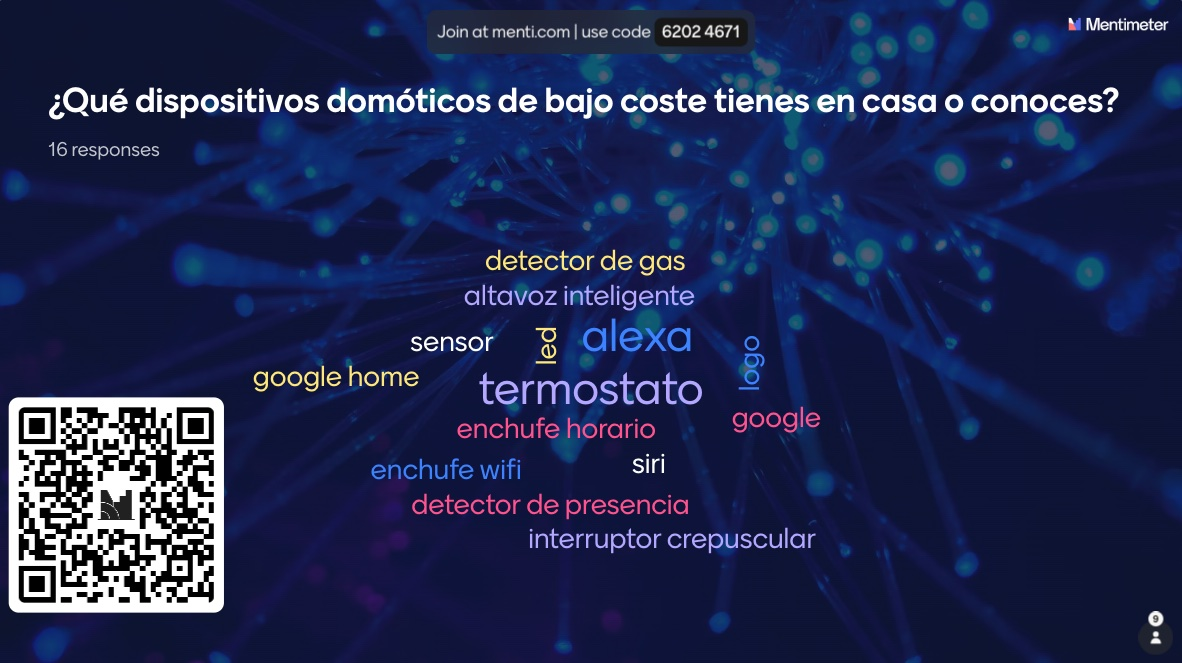
\includegraphics[width=0.8\textwidth]{resources/nube.jpg}
  \caption{Nube de palabras generada por el alumnado}
  \label{fig:nube_palabras}
\end{figure}

La actividad práctica se diseñó como una experiencia inmersiva en la que el alumnado debía simular un ataque ético. Para ello, se creó una red WiFi local con un router sin acceso a Internet, bajo el SSID “RedDomotica”, con una contraseña débil predefinida. El alumnado, trabajando en equipos, debía intentar acceder a la red, localizar un dispositivo Shelly Plug conectado, descubrir su IP y modificar su configuración sin utilizar la app oficial. 

Durante esta práctica se dieron varias situaciones destacables. Uno de los alumnos logró acceder a la configuración del router y cambió el nombre del SSID, lo que provocó que el dispositivo domótico dejara de estar accesible. Al final de la sesión, este mismo alumno se acercó a mí, algo preocupado, para confesar que había sido él quien lo había hecho, preguntando si había causado demasiados problemas. Le respondí que, si bien no era parte del plan, había sido una oportunidad valiosa para aprender de forma real y directa sobre los efectos de una mala configuración o un acceso no autorizado. 

También surgieron dificultades técnicas no previstas: no era posible acceder simultáneamente a la configuración del router desde varios dispositivos, lo cual ralentizó la actividad. Además, al intentar aplicar un ataque de fuerza bruta prolongado, el router se bloqueó temporalmente, lo que reforzó la comprensión del alumnado sobre los riesgos reales de este tipo de ataques.


% Tareas realizadas por el alumnado
\subsection{Tareas realizadas por el alumnado}

Las principales tareas que desarrolló el alumnado durante la unidad fueron:

\begin{itemize}
  \item Participación en la dinámica de nube de palabras mediante móvil y QR.
  \item Interacción durante la sesión teórica: visionado de vídeos, resolución de preguntas y debate.
  \item Acceso a la red local simulada, identificación del dispositivo conectado, análisis de su configuración y modificación del entorno.
  \item Resolución de un mini test teórico-práctico como parte de la evaluación del módulo.
\end{itemize}


% Materiales y recursos utilizados
\subsection{Materiales y recursos utilizados}

Para el desarrollo de esta unidad de trabajo se emplearon recursos didácticos, tecnológicos y materiales físicos tanto del aula como del taller del módulo de \textit{Instalaciones Domóticas}, que resultaron fundamentales para garantizar una experiencia de aprendizaje significativa y contextualizada. En un inicio, fui yo la que realizó la compra de los materiales, sin embargo, éstos no fueron utilizados, ya que el centro contaba con un router y un enchufe inteligente de la marca Shelly, que fueron los utilizados en la práctica.

Uno de los elementos clave fue el uso de un \textit{router WiFi sin conexión a Internet}, configurado previamente para crear una red local con el SSID \textit{RedDomotica}. Esta red sirvió como entorno controlado de prácticas, permitiendo que el alumnado pudiera explorar de forma segura posibles vulnerabilidades, identificar dispositivos conectados y modificar parámetros de red. La red fue diseñada con una contraseña intencionadamente débil, para facilitar la simulación de ataques de fuerza bruta y generar un contexto de reflexión sobre la importancia de una configuración segura.

El dispositivo principal de trabajo fue un \textit{enchufe inteligente Shelly Plug}, extraído del almacén del aula, junto a otros materiales domóticos disponibles en el centro. Este enchufe fue el objetivo de la práctica, permitiendo al alumnado identificar su dirección IP, acceder a su configuración y comprobar el impacto de cambios realizados desde la red local.

Además, se hizo uso de una \textit{pizarra digital interactiva SYNETECH Advance Aquarius (modelo A7532)}, adquirida recientemente por el centro gracias a fondos europeos para la modernización de la Formación Profesional. Esta herramienta facilitó la visualización de vídeos explicativos, la proyección de la presentación teórica y la generación de una \textit{nube de palabras} colaborativa a través de un código QR, permitiendo una participación dinámica e inmediata del alumnado mediante sus teléfonos móviles.

Los estudiantes utilizaron sus propios \textit{dispositivos móviles y ordenadores personales, además de los ordenadores proporcionados por el centro para los que los requerían,} para conectarse a la red local, realizar las tareas de descubrimiento y acceder a las interfaces de configuración del router y del dispositivo inteligente. Esto supuso una ventaja adicional al reproducir un entorno cercano al que podrían encontrar en un contexto doméstico real.

Por último, se diseñó una \textit{presentación en formato PDF}, que sirvió de hilo conductor para la sesión teórica. Esta incluía conceptos clave sobre seguridad, preguntas interactivas al alumnado y vídeos breves sobre vulnerabilidades en sistemas domóticos comerciales, contribuyendo a contextualizar el ejercicio práctico y fomentar una actitud crítica ante la instalación de este tipo de tecnologías.


% Criterios e instrumentos de evaluación y calificación
\section{Criterios e instrumentos de evaluación y calificación}

La evaluación de esta unidad de trabajo se diseñó conforme a un enfoque competencial, tal como establece la normativa de Formación Profesional, atendiendo no solo a la adquisición de conocimientos teóricos, sino también a la aplicación práctica, la actitud ante los retos propuestos y la reflexión crítica sobre el uso de tecnologías conectadas en red.

Los criterios de evaluación utilizados se centraron en comprobar si el alumnado era capaz de:

\begin{itemize}
  \item Reconocer riesgos de seguridad asociados a instalaciones domóticas de bajo coste.
  \item Identificar y manipular los elementos básicos de una instalación domótica (router, dispositivo conectado, red local).
  \item Aplicar medidas básicas de configuración segura, justificando sus decisiones.
  \item Verificar el funcionamiento del sistema tras la intervención.
  \item Reflexionar sobre las consecuencias de malas prácticas técnicas y éticas en entornos reales.
\end{itemize}

En cuanto a los instrumentos de evaluación, se emplearon dos. Por una parte, un análisis informal del resultado de la práctica, es decir, si el grupo había logrado acceder al dispositivo, modificar su configuración o bien reflexionar de forma crítica sobre las barreras encontradas. En este caso, no se valoró únicamente el éxito técnico, sino la comprensión del proceso y la capacidad de reflexión ante los errores. Por otra parte, se utilizó un cuestionario tipo test integrado en el examen del módulo (ver anexo \ref{examen}), que incluía tres preguntas específicas relacionadas con los contenidos y experiencias desarrolladas en la unidad. Cada pregunta valía 0,2 puntos, sumando un total de 0,6 puntos sobre la nota final del examen. Las preguntas evaluaban el conocimiento de ataques frecuentes, malas prácticas y conceptos técnicos como la escalabilidad.

Si bien no se aplicó una rúbrica formal, los criterios mencionados estuvieron presentes en el diseño de la actividad y fueron compartidos con el alumnado de manera implícita durante las explicaciones. En futuras ediciones de esta unidad se contempla la posibilidad de formalizar esta evaluación mediante rúbricas o listas de cotejo, en línea con las recomendaciones recogidas en la programación didáctica del módulo.


% Adaptaciones y atención a la diversidad
\section{Adaptaciones y atención a la diversidad}

No fue necesario aplicar adaptaciones curriculares durante esta unidad. Al tratarse de Formación Profesional, las adaptaciones curriculares de contenido no son viables, y en cuanto a las adaptaciones de acceso sólo se contemplan en casos muy concretos, y en este grupo no se dio ninguna situación que las requiriera. Sin embargo, se podría considerar como adaptación de acceso a la proporción de portátiles o materiales a los alumnos.
Tampoco se aplicaron criterios del Diseño Universal para el Aprendizaje (DUA), más allá de ofrecer información por vía visual y oral, lo cual forma parte del enfoque habitual en este tipo de módulos.
